\chapter{Síntesis lógica de un microprocesador RISC-V}
\label{ch:asp_syn}

En este capítulo se explica el proceso seguido para la sintetizar el código \textit{RTL} del microprocesador \textit{RISC-V} de aplicación específica desarrollado por el M.Sc. Carlos Salazar \cite{Carlosthesis}. En esencia la tarea encomendada consistía en efectuar la síntesis lógica del microprocesador y comprobar mediante simulaciones post síntesis su funcionabilidad.

\begin{figure}[t]
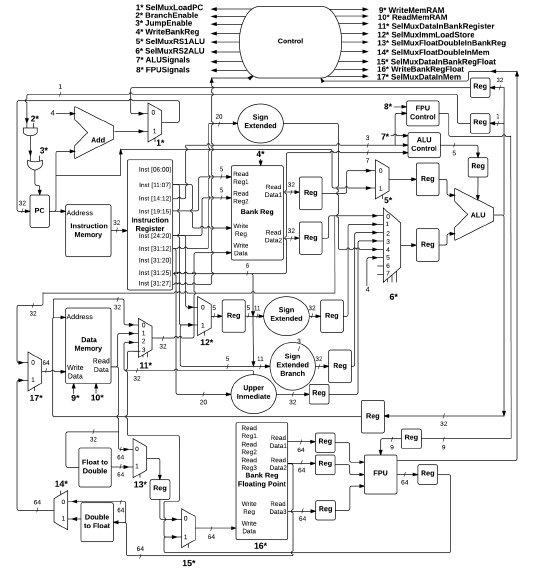
\includegraphics[width=\textwidth]{Micro.jpg}
\centering
\caption{Microprocesador ASP. RISC-V. Imágen replicada de \cite{Carlosthesis}, con la autorización del M.Sc Salazar.}
\label{fig:micro}
\end{figure}

\section{Escenario de implementación}

En la figura \ref{fig:micro}, observamos la estructura del microprocesador que debía ser síntetizado, el \textit{RTL} de este dispositivo mantiene una estructura equivalente a la de la figura \ref{fig:micro}; sin embargo, a primera impresión es posible encontrar una gran deficiencia en el diagrama de bloques mostrado. Esta deficiencia consiste en la ausencia de un hardware que permita cargarle información en las memorias. Al analizar el código del M.Sc. Salazar se encontró que las memorias utilizadas fueron definidas desde la persepectiva de ser usadas en una tarjeta de desarrollo \textit{FPGA}, este dispositivo permite cargar las memorias pues cuenta con hardware y software capacitado para dicho fin.

La estructura del \textit{RTL} de las memorias consiste en desarrollar pequeños bloques de memorias de 8 bits y generar un bloque de memoria total de 32 bits. La técnica de codificación usada corresponde a un arreglo bidimensional en verilog. En el caso de la memoria de programa o instrucciones, se crea un bloque de memoria de 32 Kbytes (kilo bytes), y se replica 4 veces para tener una memoria de 32 Kbytes con un tamaño de palabra de 32 bits, de forma similar sucede con la memoria de datos.

Sintetizar esta estructura de memorias en la herramienta es no es viable debido al enorme volumen de registros que se debe utilizar, y sin una estructura definida para guiar a la herramienta de síntesis, se obtendrá como resultado un \textit{GLN} deficiente. Es por ello que conviene incluir bloques de memoria SRAM, que correponde a una estructura de memoria más eficiente.

Considerando la meta del proyecto, la cual es desarrollar un ASIC de bajo consumo, integrar memorias tan grandes implica mal lograr el espacio de silicio disponible para el chip. Por otra parte ausencia del harware para programar las memorias compromete la correcta implementación del proyecto, pues las mismas aunque puedan ser sintetizadas por la herramienta, no podrán ser inicializadas de forma correcta, en etapas posteriores.

Existe una particularidad extra a este proyecto, y consiste en que la unidad de punto flotante original fue desarrollada por el Ing. Diego Rodríguez \cite{Diego2015}; sin embargo, el diseño tenía muchas oportunidades de mejora, es por ello que fue optimizada por el Ing. Francis López \cite{Francis2016}. Esta última no fue probada junto al microprocesador, aunque se demostró su funcionabilidad de forma individual.

Resolver los problemas asociados al banco de memoria del microprocesador y cualquier discrepancia de conectividad y sincronicidad del \textit{RTL} está más allá del alcance de este trabajo. Recordando el objetivo general de este trabajo, el cual es la implementación de un flujo de diseño digital en las herramientas de \textit{Synopsys} y para demostrar su funcionalidad se usa el \textit{RTL} del microprocesador en cuestión, es decir se pretende implementar el microprocesador ASP en una tecnología CMOS de 0,13 micrómetros, no se pretende garantizar la funcionalidad del mismo, la optimización del RTL está fuera de la visión de este trabajo.

\section{Estrategia de síntesis y validación}

Recordando, el primer objetivo específico de este trabajo, que corresponde a efectuar la síntesis lógica de el \textit{RTL} del \textit{ASP}, y habiendo definido en el capítulo \ref{ch:scripting} el flujo de diseño digital, se tiene en consecuencia que debe someterse el código \textit{RTL} a las herramientas de \textit{FrontEnd}. El flujo ya fue expuesto en el capítulo anterior, así que no se entrará en detalles sobre como fue sometido el código, pero se hablará de las configuraciones y consideraciones que se establecieron para que la implementación tenga coherencia con lo esperado del diseño.

\subsection{Restricciones del diseño}
\label{s_sec:const}

Lo expuesto a continuación corresponde a los criterios usados en el scritp de \textit{TCL} de constraints (restricciones) expuesto en la sección \ref{script_syn}. Y este es uno de los puntos de partida fundamentales para la síntesis lógica del ASP.

\subsubsection{Modelo de carga en el cableado (wire\_load\_model)}
El modelo de cableado utilizado en este diseño corresponde al ibm13\_wl10 de la biblioteca scx3\_cmos8rf\_lpvt\_tt\_1p2v\_25c. La forma para determinar los modelos de cableado se hace mediante la herramienta \textit{Design Compiler} y solicitando el reporte de la biblioteca; sin embargo, se debe tener funcionando de forma correcta el \textit{Library Compiler}. Existen varias modalidades de configuración para el modelo de cableado, en los diseños trabajados en este proyecto se utiliza el modelo "top".

En el modo superior "top", el compilador de diseño modela las redes como si el diseño no tuviese jerarquía y utiliza el modelo de carga de cable especificado para el nivel superior de la jerarquía de diseño de todas las redes en un diseño y sus subdiseños. La herramienta ignora todos los modelos de carga de cable configurados en subdiseños con el comando set\_wire\_load\_model.

\subsubsection{Reloj y factor de actividad}

Los diseños se diseñan previendo una frecuencia de operación general de 100 MHz por lo que se crea un reloj de con un periodo de 10 ns. Con el fin de modelar un reloj más realista se especifica una transición de 0.5 ns, lo cual se traduce como una pendiente en los flancos de subida y bajada del reloj.

También se específica una incertidumbre (skew) con márgenes de setup y de hold de 0.5 ns, esto corresponde al lapso entre dos flancos sucesivos con respecto a la variación fuera de los tiempos de llegada nominales. Finalmente se especifica una latencia de 0.5 ns, y es básicamente un parámetro que le indica a la herramienta el lapso que se da desde que la señal conmuta en su fuente hasta que conmuta en la entrada de una celda, y su utilidad es sólo para fines de análisis de sincronía y simulación dinámica.

Asociado indirectamente al reloj se encuentra el factor de actividad que le sirve a las herramientas, efectuar el análisis de potencia. Este parámetro se configura con una razón de conmutación del 25\% y una probabilidad estática del 50\% pues el reloj es simétrico.

\subsubsection{Puertos y propagación de señales}

Las señales de reloj y reset se configuran para que en ellas se coloquen la mínima cantidad de búfers, y que en general las señales se intervengan de forma mínima en la síntesis.

Se configura un intervalo de retraso en la propagación de los puertos, con el fin de que los análisis y la simulación sean más realistas, en el caso de las entradas el retardo es 1 ns como mínimo y de 3.5 ns como máximo, y de 1 a 2 ns para las salidas.

Los modelos de la carga asociada a las salidas y entradas se establecen en función de la celda de conducción (driving\_cell), esta configuración le permite a la herramienta de análisis de sincronía estimar de forma precisa el retraso causado desde la conmutación en un puerto, y sobre toda la ruta de propagación consecuente.

Se usa 10 la máxima cantidad de fanout permitda para los puertos de entrada, esto con el fin de que durante la síntesis la herramienta garantice que la cantidad de cargas conectadas directamente a esos puertos, no sobrepase un valor determinado.

\subsection{Comprobación de la síntesis}

Como ya se mencionó el diseño del M.Sc Salazar, presenta algunas deficiencias a la hora de considerar someterlo al flujo de diseño digital. En respuesta a lo anterior se efectuó el siguiente proceso.

\begin{enumerate}

\item En primer lugar se modificó el RTL haciendo un bypass\footnote{Bypass: anglicismo para aludir a un cambio de ruta o desvío en una ruta} en la conexión de la memorias, creando puertos para conectar de forma externa las memorias con los módulos que las instanciaban originalmente.

\item Se tomó el RTL original con la FPU diseñado por el Ing. Rodríguez, y se estimuló de acuerdo con el banco de pruebas (testbench) proporcionado junto al RTL del ASP. Esta simulación por comportamiento se define como la referencia dorada para validar el diseño.

\item Luego se sustituye la FPU por la diseñada por el Ing. López y se estimula el ASP de nuevo en una simulación por comportamiento para valorar la congruencia con el diseño original.

\item Se sintetiza entonces el RTL sin el banco de memorias, ya que como se mencionó anteriormente, incluir las memorias tal cual se diseñaron en la síntesis, es considerablemente engorroso e ineficiente.

\item Se realiza una simulación post síntesis lógica del ASP usando un estrategia de simulación hibrida, en el sentido de que se convinarán elementos de RTL (modelos por comportamiento) y elementos GLN (modelos post síntesis). Así se pretende modelar las memorias como elementos ideales y poder comprobar la funcionalidad del ASP.
\end{enumerate}

\section{Síntesis lógica del microprocesador ASP}

Habiendo definido el entorno particular en el que se recibió el RTL y las consideraciones que se tomaron para poder comprobar la correcta síntesis del mismo, se muestran los siguientes resultados ofrecidos por los reportes de la herramienta.

\begin{table}[ht]
\centering
\label{tab:qort}
\caption{QOR: Timing Path Group 'clk'}
\begin{tabular}{||l | c | c | c | c | c |}
\hline
\hline
Group & Internal & Switching  & Leakage & Total & \% Attrs \\
\hline
io\_pad & $0.0000$ & $0.0000$ & $0.0000$ & $0.0000$ & $(0.00\%)$ \\
\hline
memory & $0.0000$ & $0.0000$ & $0.0000$ & $0.0000$ & $(0.00\%)$ \\
\hline
black\_box & $0.0000$ & $0.0000$ & $0.0000$ & $0.0000$ & $(0.00\%)$\\
\hline
clock\_network & 4.0020e-02 & 0.4025 & 2.9799e+03 & 0.4425 & (35.67\%) \\
\hline
register & 0.5079 & 7.3101e-03 & 1.7763e+05 & 0.5154 & (41.55\%) \\
\hline
sequential  & 0.0000 & 0.0000 & 0.0000 & 0.0000 & (0.00\%) \\
\hline
combinational & 3.5850e-02 & 0.2464 & 3.2011e+05 & 0.2826 & (22.78\%) \\
\hline
\hline
\end{tabular}
\end{table}

% \begin{table}[h]
% \centering
% \label{tab:01}
% \caption{blablabla}
% \begin{tabular}{
% @{\hspace{0cm}}|p{1.5cm} @{\hspace{0cm}}|p{1.2cm} @{\hspace{0cm}}|p{2cm}| @{\hspace{0cm}}|p{2.2cm}|}}
% \hline
% A & B & C & D\\
% \hline
% \end{tabular}
% \end{table}







